%!TEX root = ../dissertation.tex
\section[RNA Sequencing, Differential Expression, and Descriptive Methods]{RNA Sequencing, Differential Expression, \\and Descriptive Methods}

\begin{method}

\subsection{The PREDICT Cohort}
The patient collective for the present study was recruited from a prospective, international, multi-center study with 11 study sites in Germany and Spain, led and approved by the neurologic department of Charité Berlin (www.clinicaltrials.gov, NCT01079728).\cite{Hoffmann2017} The study, called PREDICT, screened 484 stroke patients for clinical attributes and conventional biomarkers, with daily measurements in the first 5 days after stroke, and a three months follow-up. From these patients, a representative cohort of 49 patients were selected for blood small RNA sequencing. 

\subsection{Clinical Parameters Collected in the PREDICT Study}
Stroke patients were assessed daily for the duration of hospitalisation, at least until four days after admission. Blood-based biomarkers that were measured at least once during this period include: \ac{hladr}; interleukins IL-6, IL-8 and IL-10; IL-10 levels after 24h \emph{in vitro} stimulation with lipopolysaccharide; \ac{lbp}; \ac{mbl}; and \ac{tnf}-$\upalpha$. Also recorded were the time between admission and the collection of the blood sample, and the \ac{mrs}. This scale is a rough categorisation of the severity of stroke, with 0 referring to no symptoms, and 6 signifying death. Scores 1-2 describe slight neurological deficits, 3 requires frequent help because of medium level deficits, 4 requires constant assistance with daily tasks, and 5 requires stationary care.

\subsection{Sample Collection, RNA Isolation, and Sequencing}
Blood was collected into RNA stabilising tubes (Tempus Blood RNA tubes, Applied Biosystems) on each day of hospitalisation, and we subjected blood samples collected on the second day to small and large RNA-sequencing. For sequencing, we only considered samples from patients with modified Rankin Scale (mRS) values of 3 and below at discharge from the hospital, to exclude very severe cases of stroke, leaving n=240 relevant cases. The time from stroke occurrence to blood withdrawal varied between 0.94 to 2.63 days, with an average of 1.98 days. Blood samples from age- and ethnicity-matched healthy controls were obtained at matched circadian time from donors with ethical approvals from institutional review boards (ZenBio, North Carolina, USA).

RNA was extracted from 3 ml of whole blood of all 484 PREDICT patients using the Tempus Spin RNA isolation kit (Invitrogen, Thermo Fisher Scientific, Waltham MA, USA). RNA quality was determined by RNA gel for all samples and by Bioanalyzer 6000 (Agilent, Santa Clara CA, USA) for samples selected for RNA-sequencing, which showed high RNA quality with a median RIN of 8.8 (lowest RIN 7.9, highest RIN 9.9). We used 600 ng total RNA of 49 samples for small RNA library construction (NEBNext Multiplex Small RNA library prep set for Illumina, New England Biolabs, Ipswich MA, USA) and selected 24 out of the 49 short RNA-sequenced samples for PolyA-selected mRNA sequencing. These libraries were prepared from 1000 ng total RNA using the TruSeq RNA library preparation kit (Illumina, San Diego CA, USA) and were sequenced on the Illumina NextSeq 500 platform at the Hebrew University’s Center for Genomic Technologies.

\subsection{RNA Sequencing Alignment} \label{sec:stroke:alignment}
Small RNA species were aligned after quality filtering using flexbar and miRExpress 2.0, as described in Section \ref{sec:cellculture:alignment}. Additionally, to assess tRF expression, small RNA reads were aligned to the exclusive tRNA space using the MINTmap pipeline.\cite{Loher2017} Briefly, this pipeline compares short RNA sequencing reads with a collection of sequences determined to only be contained inside mature tRNAs, without confounding from the many tRNA lookalikes in the human genome, e.g., in pseudogenes. The two RNA species were united into one expression matrix containing both miRNA and tRF expression.

Large RNA species were aligned to the human transcriptome using the ENSEMBL transcriptome \emph{Homo sapiens} GRCh38 release 79, and using the fast dual-phase parallel inference algorithm \emph{Salmon}.\cite{Patro2017} \emph{Salmon} combines an »online« fragment mapping utilising continuous updating of a Bayesian prior with an »offline« phase that determines fragment quantities by application of the Bayesian model determined before via a standard expectation maximisation (EM) algorithm or a variable Bayesian EM. Additionally, the pipeline corrects for multiple typical biases in sequencing, such as position-specific biases, sequence-specific 3' and 5' end biases, fragment GC content bias, and fragment length distribution. The resulting quantified fragments were imported into R using the rsubreads package.\cite{Liao2019}

\subsection{Quality Control and Filtering}
Raw and processed reads were quality-controlled using FastQC, as described in Section \ref{sec:cellculture:sequencing}, with no samples falling below acceptable thresholds. Small and large RNA alignments were batch-corrected followed by analysis of inter-sample relationships via the method proposed by Oldham \emph{et al.}\cite{Oldham2012} (as described in Section \ref{sec:cellculture:quality}). We excluded no large RNA samples and one small RNA sample (»11\_40044\_S12«).

\subsection{RNA Sequencing Differential Expression Analysis}
Quantified reads were subjected to differential expression analysis using DESeq2, essentially as described in Section \ref{sec:cellculture:deseq}. Small RNA species were analysed together by combining count tables for miRNAs and tRFs, large RNAs were analysed separately. Both datasets were corrected for covariates \emph{subject age} and \emph{batch}. Correction for patient sex was not necessary because all patients in the final analyses were male. \ac{lfc} values were shrunk using \emph{apeglm} as described in Section \ref{sec:cellculture:deseq}, at an alpha level of \emph{0.1}.

\subsection{Gene Ontology Analyses}
We performed \ac{go} analyses on the set of \ac{de} transcripts, using different ranking methods. GO analyses were performed using R/topGO as described in Section \ref{sec:cellculture:topgo} using the weighted method.

\subsubsection{Ranking by P-Value}
Transcripts were ranked by p-value, and different test sets were tested against the background of the topmost two thousand transcripts. We tested the set of all \ac{de} transcripts (adjusted p-value < 0.05) and the separate sets of positively and negatively regulated transcripts. Additionally, for each test group, the criterion of \ac{lfc} > 1.4 was applied and re-tested.

\subsubsection{Ranking By Count-Change}
Alternatively to ranking via p-value, transcripts were ranked by count-change, and the top 100 significantly \ac{de} transcripts were tested against the background of the first two thousand transcripts. Similarly to the p-value ranking, test sets comprised all transcripts as well as only negatively or positively regulated transcripts.

\subsubsection{Visualisation of Results}
While GO enrichment analysis can be informative, interpretation and visualisation of its results is not standardised and often limited to presentation of top \emph{X} terms by p-value. R/gsoap\cite{Tokar2020} is an analysis tool proposed to aid in interpretation of GO enrichment results via \acf{tsne} display of similarity of terms based on the amount of shared significant genes. GO enrichment results were processed to fulfil \emph{gsoap} input criteria and visualised using \emph{ggplot2}.\cite{Wickham2016}

\subsection{Homology Computation Among tRNA Fragments}
Transfer RNA fragment origin can be ambiguous, even in fragments derived from tRNA-exclusive space. To assess sequence-based relationships between tRFs, all detected fragments were subjected to pairwise homology analysis using local Smith-Waterman alignment (\emph{pairwiseAlignment} function of the R/Biostrings package), and scores were transformed into a distance matrix to enable clustering and visualisation of relationships. \ac{tsne} was employed to visualise tRF homologies in a 2D space.

\subsection{t-Distributed Stochastic Neighbour Embedding} \label{sec:stroke:tsne}
SNE (Stochastic Neighbour Embedding) replaces Euclidian distances between data points with conditional probabilities that represent similarities. The Gaussian distribution used in SNE to represent the probability density for any given data point in the low-dimensional space is replaced by a Student's t-Distribution in the updated \ac{tsne} algorithm. In combination with the use of a symmetrised function with simpler gradients, this alleviates problems with optimisation of the cost function that is used to create forces between points on the low-dimensional map.\cite{Maaten2008} The superiority of \ac{tsne} with random initialisation remains subject of debate, and some advocate the use of the newer UMAP algorithm\cite{McInnes2018}, although most of the discussion is centered around analysis of single-cell \ac{seq} and preservation of global structure in the lower-dimensional visualisation.\cite{Becht2019}

\ac{tsne} was used in a variety of applications to reduce the dimensionality of high-dimensional data, for instance, the amino acid origin of tRFs, or the association of tRFs with distinct cell types in the blood. \ac{tsne} analyses were performed in R, using the Rtsne package.\cite{Krijthe2015} \ac{tsne} requires, apart from the input data, a parameter called \emph{perplexity}, which determines the weighting of local as opposed to global effects in the data. So far, there are no strict rules governing the selection of a perplexity value, other than that the perplexity cannot exceed the number of individual data points. Since different perplexities can give widely varying results, which can sometimes be misleading, the resulting maps have to be screened with a range of perplexities to assess their robustness.

\subsection{Cholinergic Association of Small RNA Species} \label{sec:stroke:chol-assoc}
To determine association of distinct smRNAs with cholinergic transcripts, we analysed the multiple-targeting relationships of each distinct smRNA towards our curated list of \ac{ca} transcripts. We first created complete targeting data of all DE smRNAs towards all \ac{ca} transcripts, which we then successively filtered for multiple targeting behaviours. To assess the base level of multiple targeting of cholinergic transcripts, we utilised empirical cumulative density functions of the number of individual cholinergic targets of each miRNA and tRF (Figure \ref{fig:cholino-ecdfs}). We assumed 80\% to be a robust threshold of cholinergic targeting, and for diverging numbers between miRNAs and tRFs chose to use the higher (more stringent) threshold. smRNAs above this threshold (i.e., smRNAs targeting at least as many cholinergic transcripts as the threshold value) were considered \ac{ca}.

\end{method}

\begin{figure}
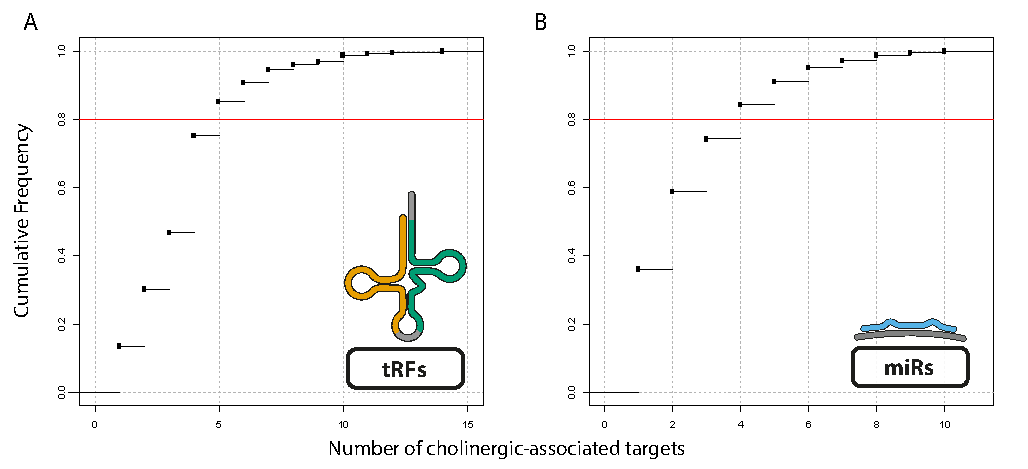
\includegraphics[width=\textwidth]{figures/cholino-ecdfs}
\caption[Cholinergic-associated Small RNA ECDF Curves.]{\textbf{Cholinergic-associated Small RNA ECDF Curves.} Cholinergic association was tested using \emph{miRNeo} targeting data of miRNAs and tRFs. To assess the best-suited threshold for defining cholinergic association, empirical cumulative density functions were calculated for the number of \acf{ca} genes targeted by each unique smRNA. \textbf{A)} Cumulative frequency of number of \ac{ca} genes targeted by tRFs. Threshold of 80\% (red line) is passed at five \ac{ca} genes targeted. \textbf{B)} Cumulative frequency of number of \ac{ca} genes targeted by miRNAs. Threshold of 80\% (red line) is passed at four \ac{ca} genes targeted.
\label{fig:cholino-ecdfs}}
\end{figure}

\newpage

\section[Descriptive Analysis of RNA Dynamics in Blood After Stroke]{Descriptive Analysis of RNA Dynamics \\in Blood After Stroke}

\subsection{Differential Expression of Large RNA} \label{sec:stroke:mrna}
At an alpha level of 0.05, we detected 694 \acf{de} long transcripts, 204 of them up- and 490 down-regulated (Figure \ref{fig:stroke-de-tsne}\,A). 18 of the up-regulated and 109 of the down-regulated transcripts exceeded the common \acf{lfc} threshold of 1.4. To determine the most-impacted pathways, we performed \ac{go} analyses.

\subsection{Gene Ontology Analyses of Differentially Expressed Genes} \label{sec:stroke:large-rna-go}
Ranking of all transcripts (regardless of direction of regulation) by their differential expression p-value resulted in GO terms mainly related to circulatory system processes (p = 0.018) and immunity (Figure \ref{fig:gsoap-de}\,A). Most notable immune-related terms included cytokine-mediated pathways (p = \e{2.4}{-4}), response to \acp{ifn} $\upalpha$ (p = 0.013) and $\upbeta$ (p = \e{1.2}{-3}), regulation of JAK/STAT cascade (p = 0.013), response to \ac{lps} (p = 0.025), and macrophage activation (p = 0.026). Limiting the test set to transcripts with \ac{lfc} above 1.4\,\,increased sensitivity towards immune processes, yielding lower p-values for the enrichment of of positive (\e{1.7}{-4}) and negative regulation of cytokine production (\e{5.7}{-4}), type I interferon production (\e{3.9}{-4}), response to bacterium (\e{5.9}{-4}), innate immune response (\e{2.0}{-3}), response to organophosphorous (\e{2.3}{-3}), cytoplasmatic pattern recognition receptor signalling pathway (\e{2.8}{-3}), and response to \ac{lps} (\e{9.1}{-3}).

Up-regulated transcripts pertained to circulatory system processes, such as platelet degranulation (\e{1.2}{-3}) and aggregation (0.02), and sprouting angiogenesis (\e{4.8}{-3}), but also antigen processing and presentation (\e{4.5}{-3}). Test set limitation to \ac{lfc} above 1.4 did not increase sensitivity towards those terms, but presented essentially similar results. Up-regulated genes as such may be indicative of the bodily response to blood flow disruption and ischaemia caused by the stroke. 

Down-regulated transcripts were enriched in terms involving response to \ac{ifn} $\upalpha$ (\e{1.3}{-3}) and $\upbeta$ (\e{3.1}{-4}), response to \ac{lps} (\e{1.5}{-3}), rhythmic process (\e{2.5}{-3}), positive regulation of T cell proliferation (\e{4.3}{-3}), positive regulation of JAK-STAT cascade (0.015), and cellular response to \ac{il}-1 (0.019). Test set limitation to \ac{lfc} above 1.4 again increased sensitivity towards immune-related terms, but without changing the general pattern. Thus, down-regulated genes in all likelihood represent the post-stroke immunodepression, which can exacerbate into CIDS (see Section \ref{sec:intro:stroke}). The terms involving INF, IL-1, LPS, and JAK-STAT also indicate an important role for cytokine signalling in these processes.

\begin{figure}
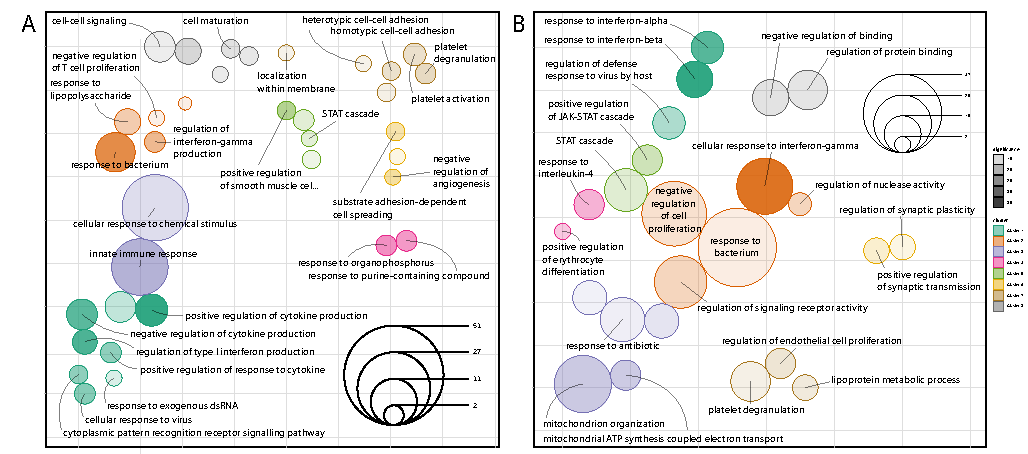
\includegraphics[width=\textwidth]{figures/gsoap-de}
\caption[Large RNA Differential Expression Gene Ontology Enrichment.]{\textbf{Large RNA Differential Expression Gene Ontology Enrichment.} GO terms from enrichment analysis were projected on a 2D map via \acf{tsne} analysis of their shared significant genes. LEGEND \textbf{A)} \ac{tsne} visualisation of GO terms of DE genes with \ac{lfc} > 1.4 shows 36 terms in eight clusters. Immunological terms (left-hand side) and circulatory terms (right-hand side) are predominant. \textbf{B)} \ac{tsne} visualisation of 24 GO terms of top 100 genes measured by count-change corroborate immunological changes in stroke patient blood differential gene expression.
\label{fig:gsoap-de}}
\end{figure}

As a cross-check, \ac{de} transcripts were ranked by count-change, and re-analysed (Figure \ref{fig:gsoap-de}\,B). The top 100 changed transcripts, without regard to direction (absolute count-change) yielded terms implying response to \ac{ifn} $\upalpha$ (\e{3.8}{-4}), $\upbeta$ (\e{1.1}{-4}), and $\upgamma$ (\e{1.4}{-4}), mitochondrial organisation (\e{5.6}{-3}) and ATP synthesis (\e{6.9}{-3}), response to \ac{il}-4 (\e{6.9}{-3}), positive regulation of JAK-STAT cascade (\e{8.8}{-3}), response to antibiotic (0.044), and platelet degranulation (0.045). The top 100 up-regu"-la"-ted transcripts yielded terms involving platelet degranulation (\e{3.8}{-3}), mitochondrial ATP synthesis (\e{4.2}{-3}), response to xenobiotic stimulus (0.017), platelet aggregation (0.013), and response to antibiotic (0.016), while the top 100 down-regulated transcripts were associated with inflammatory response (\e{1.3}{-4}), regulation of apoptosis (\e{1.8}{-4}), cytokine secretion (\e{6.8}{-4}), antigen processing and presentation (\e{1.2}{-3}), regulation of lymphocyte apoptosis (\e{2.3}{-3}) and proliferation (\e{2.7}{-3}), response to antibiotic (\e{5.2}{-3}), leukocyte homeostasis (\e{7.6}{-3}), response to \ac{il}-1 (\e{7.6}{-3}), and many more immune-specific processes. This corroborates the previous findings that up-regulated transcripts represent the response to circulatory system damage, and down-regulated transcripts indicate a cytokine-mediated immunodepression. For a full list of all terms from these analyses, see Appendix \ref{appendix:go-terms-large-rna}. 

\subsection{Differential Expression of small RNA}
In the simultaneous co-analysis of miRNAs and tRFs, we detected 420 DE miRNAs and 143 DE tRFs (adjusted p-value < 0.05, Figure \ref{fig:stroke-de-tsne}\,B\&C). 63\% of miRNAs (265) were down-regulated, while 87\% of tRFs (124) were up-regulated. tRFs were mainly derived from the 3' end (3'-tRFs, 87) or from internal tRNA regions (i-tRFs, 48), while the tRFs from 5' ends (5'-tRFs) were in the minority (6). The amino acid distribution was shifted in favour of alanine- (35), glycine- (28), and proline-carrying (12) tRNAs (Figure \ref{fig:stroke-de-tsne}\,D). 30 of the 35 alanine-associated tRFs were 3'-tRFs, and all of those were up-regulated, indicating non-random generation of these fragments.

\begin{figure}[ht]
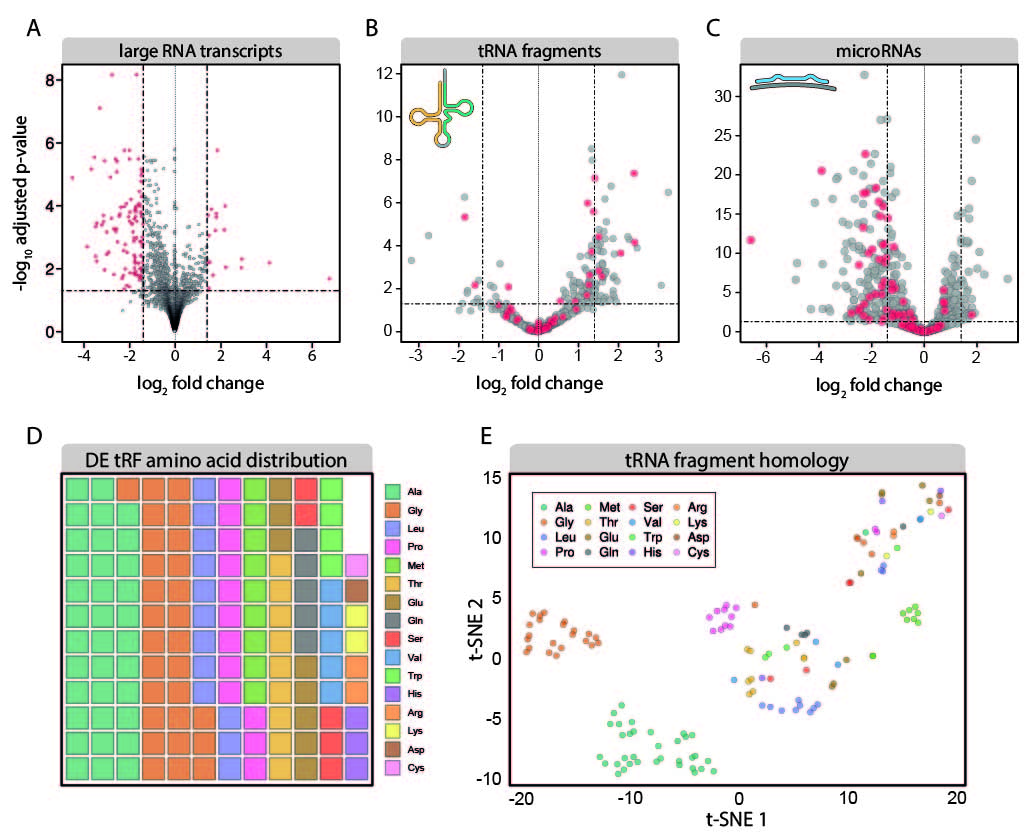
\includegraphics[width=\textwidth]{figures/stroke-de-tsne}
\caption[Small and Large RNA Differential Expression and tRF Properties.]{\textbf{Small and Large RNA Differential Expression and tRF Properties.} \textbf{A)} Differential expression analysis reveals multiple large RNA transcripts changed in patient blood after stroke. The majority of differentially expressed (DE) transcripts above a \ac{lfc} threshold of 1.4 (red) are down-regulated. \textbf{B)} Blood-borne tRNA fragments (tRFs) also change after stroke. Unlike large RNA and miRNAs, the majority of DE tRFs are up-regulated. \Acf{ca} tRFs in red. \textbf{C)} Blood-borne miRNAs are heavily influenced by the events following stroke. Like large RNA transcripts, miRNAs are also overwhelmingly down-regulated. \Ac{ca} miRNAs in red. \textbf{D)} The distribution of amino acid origin among the DE tRFs is non-random and biased towards the amino acids alanine, glycine, leucine, proline, and methionine. Each square represents one DE tRF, colour denotes amino acid origin. \textbf{E)} \acf{tsne} of pairwise fragment homology by local Smith-Waterman alignment shows clustering of the dominant amino acid groups of tRFs. Clear clusters can be observed for tRFs derived from tRNA carrying alanine, glycine, leucine, proline, and methionine.
\label{fig:stroke-de-tsne}}
\end{figure}

\subsection{Homology Among tRNA Fragments}
Using pairwise homology among all DE tRFs, visualised via \ac{tsne} (see Section \ref{sec:stroke:tsne}), we identified clusters of highly similar fragments, that correlate with their amino-acid origin, i.e., the amino acid which is carried by the respective parent tRNA (Figure \ref{fig:stroke-de-tsne}\,E). This relationship persisted across distinct individual tRNAs coding for the same amino acid, and was particularly pronounced in tRNAs associated with alanine, glycine, leucine, proline, and methionine. This further indication of non-random generation of tRNA fragments shorter than tiRNAs leaves an open question about their biogenesis, particularly, which nucleases are responsible for the generation of the mature transcripts, and if 3'-tRF generation is dependent or independent from tiRNA generation by angiogenin.

\subsection{Cholinergic Association of Small RNA Species}
The association of smRNA species to distinct systems or pathways is not trivial because of the multiple-targeting nature of these RNAs. For the purpose of the following analyses, we defined a small RNA as being associated with cholinergic processes by the positive association of the smRNA with a number of \acf{ca} large transcripts. We did not assess the question whether this small RNA also targeted other systems equally, or if it targeted cholinergic transcripts with greater likelihood than a random selection of genes. For this reason, we selected a fairly high threshold for the definition of a \ac{ca} smRNA, which is the targeting of at least 5 \ac{ca} transcripts (above 80\% on the empirical cumulative density function of cholinergic targeting, see Section \ref{sec:stroke:chol-assoc}).

Following this definition, we detected 52 \ac{ca} miRNAs (90\% down-regulated, 5 up and 47 down), and 18 \ac{ca} tRFs (83\% up-regulated, 15 up and 3 down). Above an \ac{lfc} threshold of 1.4, we found 33 \ac{ca} miRNAs (97\% down-regulated, 1 up and 32 down), and 9 \ac{ca} tRFs (78\% up-regulated, 7 up and 2 down). \ac{ca} smRNAs are marked in red in Figure \ref{fig:stroke-de-tsne}\,B\&C.

\newpage
